\section{Dijkstras algoritme}
I \ref{defn:min.vej} definerede vi distancen af den korteste vej i en vægtet graf. For at finde den korteste vej vil vi anvende \emph{Dijkstras algoritme}. Dijkstras algoritme kan bruges til at finde den korteste vej i en simpel, vægtet graf, hvori vægtene for alle kanter i grafen skal være ikke-negative. Algoritmen fungerer således, at den finder den korteste vej fra en startknude, $v_{1}$, til en endeknude, $v_{m}$, ved først at finde naboknuderne til $v_{1}$ og undersøge hvilken af disse, der har den mindste distanceværdi og altså er tættest på startknuden. Derefter tager den udgangspunkt i den naboknude, hvortil distanceværdien er mindst og fortsætter ad dennes vej, så længe denne vej har en mindre distanceværdi end en alternativ vej. Fremgangsmåden vil her illustreres ved hjælp af et eksempel, som tager udgangspunkt i \ref{kap:grafteori}.

\begin{exmp}
Betragt figur \ref{fig.dijkstraexmp}
\begin{figure}[H]
\centering
	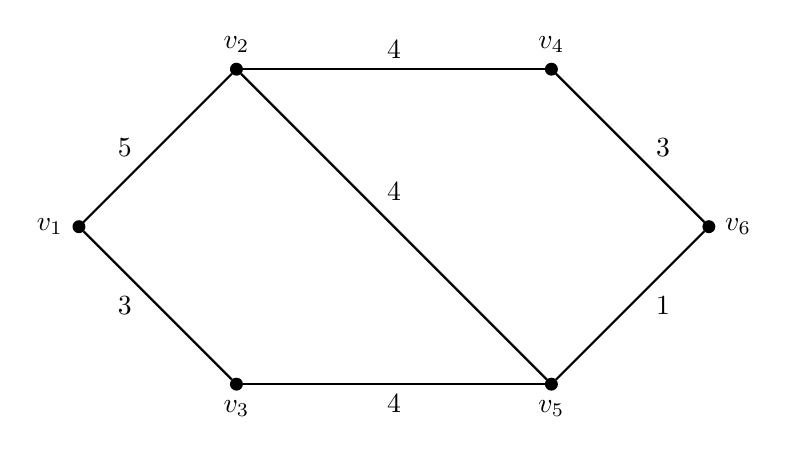
\begin{tikzpicture}

      \tikzset{enclosed/.style={draw, circle, inner sep=0pt, minimum size=.15cm, fill=black}}
%% Vertices
      	\node[enclosed, label={left: $v_1$}] (v1) at (0,2) {};
      	\node[enclosed, label={above: $v_2$}] (v2) at (2,4) {};
    	\node[enclosed, label={below: $v_3$}] (v3) at (2,0) {};
  	    \node[enclosed, label={above: $v_4$}] (v4) at (6,4) {};
     	\node[enclosed, label={below: $v_5$}] (v5) at (6,0) {};
     	\node[enclosed, label={right: $v_6$}] (v6) at (8,2) {};
%Edges
		\path [-, > = latex, thick] (v1) edge node[midway, left=2mm] {$ 5 $} (v2);
		\path [-, > = latex, thick] (v1) edge node[midway, left=2mm] {$ 3 $} (v3);
		\path [-, > = latex, thick] (v2) edge node[midway, above] {$ 4 $} (v4);
		\path [-, > = latex, thick] (v2) edge node[midway, above=2mm] {$ 4 $} (v5);
		\path [-, > = latex, thick] (v3) edge node[midway, below] {$ 4 $} (v5);
		\path [-, > = latex, thick] (v4) edge node[midway, right=2mm] {$ 3 $} (v6);
		\path [-, > = latex, thick] (v5) edge node[midway, right=2mm] {$ 1 $} (v6);

	\end{tikzpicture}
	\caption{Simpel, vægtet graf.}
	\label{fig.dijkstraexmp}
\end{figure}
I figur \ref{fig.dijkstraexmp} vil vi finde den korteste vej fra $v_{1}$ til $v_{6}$. Dijkstras algoritme vil gøre dette ved at finde den korteste vej fra startknuden, $v_{1}$, til hver knude, indtil den når endeknuden, $v_{6}$. Først vil den se, at startknuden har naboknuderne $v_{2}$ og $v_{3}$. Der er altså to veje fra startknuden, $P=(v_{1},v_{2})$ med distancen 5 og $P=(v_{1},v_{3})$ med distancen 3. Dermed er $v_{3}$ den knude, der er tættest på startknuden. Herefter er der igen to veje, $P=(v_{1},v_{2})$ med distancen 5 og $P=(v_{1},v_{3},v_{5})$ med distancen 7. Den første af disse vælges, da denne har den mindste distance, og $v_{2}$ er dermed knuden, som er næsttættest på startknuden. Nu er der tre forskellige veje, $P=(v_{1},v_{2}, v_{4})$ med distancen 9, $P=(v_{1},v_{2}, v_{5})$ med distancen 9 og $P=(v_{1},v_{3}, v_{5})$ med distancen 7. Den tredje vælges, og det er nu noteret, at den korteste vej fra $v_{1}$ til $v_{5}$ har distancen 7. Der er nu igen kun to mulige veje at vælge imellem, $P=(v_{1},v_{2}, v_{4})$ med distancen 9 og $P=(v_{1},v_{3}, v_{5}, v_{6})$ med distancen 8. $P=(v_{1},v_{2}, v_{5})$ er ikke længere en mulig vej, da vi allerede har fundet den korteste vej fra $v_{1}$ til $v_{5}$. Den anden vej har den mindste distance, og derfor vælger vi denne, og vi ved nu, at den korteste vej fra $v_{1}$ til $v_{6}$ er $P=(v_{1},v_{3}, v_{5}, v_{6})$ og har distancen 8.
\end{exmp}
Ovenstående eksempel er simpelt og kan hurtigt løses ved fx brute force metoden, men i større og mere komplicerede grafer er Dijkstras algoritme meget mere effektiv. For at skabe yderligere overblik over hvordan Dijkstras algoritme fungerer, vil vi her gå i dybden med dennes mere teoretiske del.
\begin{algorithm}[H]
\caption{Dijkstras algoritme}
\begin{algorithmic}[1]

\Procedure{dijkstra($G$: vægtet, sammenhængende, simpel graf med kun ikke-negative vægte)}{}
    \State \{$G$ {har knuderne $a = v_{1}, v_{2}, \dotsc, v_{m} = z$ og vægtene til kanterne $w(v_{i}, v_{j})$, hvor $w(v_{i}, v_{j}) = \infty$ hvis $v_{i}$ og $v_{j}$ ikke er naboer \}}
	\For {$i := 2$ \textbf{to} $m$}
		\State $L(v_{i}) := \infty$
	\EndFor
	\State $L(a) := 0$	
	\State $S := \emptyset$
	\State {\{distancen til hver knude initialiseres, så $a = 0$, og distancen til alle andre knuder er $\infty$, derudover er $S$ defineret som en tom mængde\}}
    \While{$z \notin S$}
        \State {$u :=$ en knude som ikke er i $S$ med $L(u)$ som minimum}
        \State $S := S \cup \{u\}$
        \For {alle $v \notin S$}
        	\If {$L(u) + w(u,v) < L(v)$} {$L(v) := L(u) + w(u,v)$}
        	\State \{dette tilføjer knuder til $S$ med minimal 			distance og opdaterer distancerne til
        	\State knuderne, som ikke er i $S$\}
        	\EndIf
    	\EndFor
    \EndWhile
    \State {\textbf{return} $L(z)$ \{$L(z) = \alpha(a,z)$\}} 
\EndProcedure

\end{algorithmic}
\label{alg:dijkstra}
\end{algorithm}
Det første, der sker, er, at startknuden noteres som $0$, altså $v_{1} = 0$, og resten af knuderne noteres som $\infty$. Her betegnes den korteste vej som $\alpha_{k}(v_1,v_m)$, fra definition \ref{defn:min.vej}, hvor $k$ er antallet af \emph{iterationer} gennemført i algoritmen. Antallet af iterationer er det antal gange en løkke gennemkøres, altså hver gang vejen opdateres.  $\alpha_{0}(v_1,v_1)$ betyder altså, at vi har nul iterationer og dermed kun kender startknuden med distancen 0. Derudover oprettes en mængde $S$, for hvilken det gælder, at $S = \emptyset$ når $k = 0$. Ved første iteration undersøges startknudens naboknuder, og man bestemmer, som i eksemplet ovenfor, hvilken distance er mindst. Dermed er startknudens nærmeste knude fundet, og denne tilføjes nu til mængden $S$. For hver iteration tilføjes et nyt element til mængden, og denne proces fortsætter, til algoritmen har fundet den korteste vej fra startknuden til endeknuden. Mængden, $S$, indeholder til sidst distancerne for den korteste vej fra startknuden til alle knuder i grafen. 


